\documentclass[11pt]{article}
\usepackage[letterpaper,margin=1in]{geometry}
\usepackage{amsmath,amssymb,amsthm,mathtools}
\usepackage{graphicx,booktabs,array,tabularx}
\usepackage{natbib,microtype,placeins,caption}
\usepackage[hidelinks]{hyperref}
\captionsetup{font=small,labelfont=bf}
\setlength{\parskip}{0.25em}
\setlength{\emergencystretch}{1.5em}
\renewcommand{\arraystretch}{1.15}
\clubpenalty=10000
\widowpenalty=10000
\displaywidowpenalty=10000
\brokenpenalty=10000
\newtheorem{theorem}{Theorem}
\newtheorem{proposition}{Proposition}
\newtheorem{lemma}{Lemma}
\newtheorem{definition}{Definition}
\newtheorem{corollary}{Corollary}
\newcommand{\Fleet}{\mathcal F}
\newcommand{\Loads}{\mathcal L}
\newcommand{\R}{\mathbb R}
\let\originalsection\section
\renewcommand{\section}{\FloatBarrier\originalsection}
\let\originalsubsection\subsection
\renewcommand{\subsection}{\FloatBarrier\originalsubsection}
\title{Marginal-price support and repeated optimization\\of electric-bus fleets}
\author{}
\date{Research draft 0.6 for author review --- 28 September 2026}
\begin{document}
\maketitle
\begin{abstract}
Electric-bus charging combines continuous energy decisions with indivisible service assignments. We study whether a complete feasible fleet schedule is a best response to the marginal electricity prices generated by its own load. An exact, fully replenished two-service construction exhibits a positive gap between physical and convexified planning, with a robustness neighborhood allowing charging losses, a reserve and a finite connector. In a replication family, the absolute planning gap vanishes while whole-operator regret remains positive along a subsequence; regret per reserved pair vanishes. Computational development studies then examine repeated complete-fleet optimization on two synthetic cases and two depot variants of one public timetable. Reusing feasible fleets and physical-pricing bounds improves particular bounds, but public optimality gaps remain open and native starting-fleet effects are mixed. We separate feasible dispatch, convex mixtures, numerical certification and paid computation. These results motivate further proposal-based acceleration without establishing a speedup or a learned scheduling method.
\end{abstract}
\noindent\textbf{Keywords:} electric-bus scheduling; convex-hull pricing; marginal tariffs; charging coordination; repeated optimization.

\section{Introduction}
An electric-bus operator must cover mandatory passenger services while assigning vehicles and scheduling charging. A tariff can shift charging toward cheaper periods, but a fleet large enough to affect aggregate electricity demand also changes the marginal cost behind that tariff. Even with continuously adjustable charging, its service assignments remain indivisible. The resulting question is whether a physically realizable fleet schedule minimizes the operator's bill when evaluated at the marginal prices associated with that schedule's load.

We study this question using complete fleet plans. Each plan includes all services, vehicle movements, charging and operating cost. Convexifying their joint cost and load vectors provides a useful planning lower bound, but a point in that hull is generally not an executable daily dispatch. Charging a convex supply cost at the mean load also differs from taking the mean cost of randomized physical dispatches. Maintaining these distinctions is essential both for interpreting a pricing failure and for assessing computational shortcuts.

The contribution has two parts. First, a small continuous-charging construction makes the obstruction explicit under full terminal replenishment. A perturbation permits a positive reserve, charging losses and one finite connector. A replication calculation then separates an aggregate planning gap from the incentives of a whole-fleet operator and of participants with individually reserved resources. These are application-specific exact results within established nonconvex pricing theory, rather than a new general decentralization theorem. Second, development computations ask what repeated optimization can reuse, and what still requires global physical-fleet pricing. Their tables expose both useful bounds and incomplete solves.

The computational scope is deliberately stated at the level observed: two small synthetic diagnostics and two depot variants of one public timetable. The campaigns share cases and some source evidence; they are not independent replications across transport networks. Their clearest findings concern particular bound improvements and the cost of fresh physical pricing. They do not demonstrate public-case global optimality, a general speedup at equal quality, or learned route prediction. This manuscript therefore provides an exact mechanism and a computational foundation for a broader study, with the remaining empirical questions explicit.

\section{Related work}

Electric-bus scheduling jointly assigns service to vehicles and tracks battery and charging decisions. Wu et al. study multi-depot scheduling with grid objectives; de Vos et al. model partial charging and station capacity; Parmentier et al. scale route and recharge scheduling by column generation \citep{wu2022grid,devos2024capacity,parmentier2023fleets}. These works establish operational roles for duty construction, energy limits, and charging resources. Here we ask how a complete fleet plan relates to the convex hull of complete plans under a common convex supply-cost model. A duty-column relaxation need not equal this whole-fleet hull, and a mean load in the hull need not be executable as one day's bus schedule.

Public timetable and movement data make this distinction testable without fixing the economics. Sistig et al. generate bus and crew schedules for twenty German transport networks from public GTFS inputs; their versioned dataset includes routes, trips, stops, possible deadheads, and schedules \citep{sistig2025dataset,sistig2025electrification}. We use one Hildenbrand timetable in two restricted depot variants. Source distances, times, and bus parameters are combined with EGG's declared energy, battery, reserve, charger, horizon, and synthetic convex supply-cost assumptions; the dataset supplies no EGG market-supply function. These remain small development studies on one timetable and two depots, with public global bounds open. They establish neither an equal-quality speedup nor a learned-proposal benefit.

Nonconvex electricity-market research explains why marginal prices can fail to support dispatch with indivisible operating decisions. Gribik et al. compare unit-commitment pricing rules and discuss energy uplift when no energy-price vector supports selected quantities \citep{gribikHoganPope2007}; O'Neill et al. construct prices from a mixed-integer model and associated linear program \citep{oneill2005}. Convex-hull pricing studies uniform prices through convexification: Schiro et al. discuss its formulation and implementation, and Hua and Baldick give a convex primal formulation \citep{schiro2016,huaBaldick2017}. Madani et al. compare convex-hull, integer-programming, and European-style pricing with nonconvex demand bids; Andrianesis et al. compute convex-hull prices by Dantzig--Wolfe decomposition and column generation \citep{madani2018pricing,andrianesis2022hull}. Hümbs et al. characterize linear-price support for decentralized problems with integralities and complete linear feasible-set descriptions \citep{huembs2022complete}. These are precedents for convex-hull pricing and price-support questions; we use the same general supporting-price logic for a stated fleet set and supply-cost function. Our own-price best-response test is conditional on that model, not a general market-clearing theorem or settlement design; fleet regret is not an uplift payment under these market rules.

Aggregation results also require their own scale and participant definitions. Starr's classical quasi-equilibrium result gives an aggregation perspective for economies with nonconvex preferences \citep{starr1969}. Our replication construction is proved directly for its specified fleet schedules: the aggregate planning gap tends to zero while whole-operator regret can remain positive, whereas per-bus and individually reserved-pair incentives vanish. A Shapley--Folkman aggregation argument does not by itself prove this exact replication result or force the absolute regret of one composite operator to vanish. The distinction is between aggregating many separately bounded participants and enlarging a single participant whose opportunity set remains indivisible.

Price coordination for flexible EV charging is established. Gan et al. model each vehicle's charging profile as a continuous, rate-bounded vector with fixed energy over an availability window and give a price-update protocol converging for a convex aggregate-load objective \citep{ganTopcuLow2013}. This coordinates charging once availability and energy needs are fixed. Bus schedules additionally assign trips to vehicles, changing charging windows and the joint feasible load set. Convex charging coordination therefore does not imply own-price support for a discrete complete bus schedule.

Fixed-schedule fleet counting has a classical analogue in Dantzig and Fulkerson's minimum-tanker problem \citep{dantzigFulkerson1954}. Such flow reductions count vehicles covering fixed movements, but do not certify battery states, shared-charger feasibility, or price support. We separate minimum-fleet flow diagnostics, charging replay, and convex-hull economic comparisons.

\section{Complete fleets and marginal-price support}\label{sec:model}

The unit of optimization is a \emph{complete} fleet plan, rather than an
individual vehicle duty.  Fix a timetable, allowed directed movements, a
charging horizon, and the equipment and energy assumptions.  Let
$\Fleet\ne\varnothing$ contain precisely the plans that cover every mandatory
service once, assign the services to used buses, route those buses through
allowed movements, respect battery and charger constraints, and restore every
used bus to its required terminal inventory.  For $x\in\Fleet$, write $c(x)$
for intrinsic operating cost and $e(x)\in\R_+^T$ for grid energy bought in the
$T$ market intervals.  An unused bus contributes neither charging nor cost.
We use the same $\Fleet$, $c$, and $e$ for physical planning, price response,
and convexification.  Finitely many discrete duties with bounded continuous
charging give a compact $\Fleet$ in the cases below; assume more generally
that its image $\{(e(x),c(x)):x\in\Fleet\}$ is compact.

In the timed physical model, each used path starts at battery inventory $B$.
A service or directed movement consumes its declared energy in chronological
order.  Inventory remains between reserve $r$ and capacity $B$ at every
event.  A depot charging session buying $q$ grid kWh adds $\eta q$ inventory,
where $0<\eta\leq1$, within its availability window and bus-power limit.
Concurrent sessions obey the shared power or connector limit.  Each path
finishes at inventory $B$ by the declared horizon.  In the homogeneous
single-connector formulation, charging intervals are split at all visit and
market boundaries.  If interval $k$ has duration $d_k$ and power $P_k$, its
charges obey $0\leq z_{mk}\leq P_kd_k y_m$ and
$\sum_m z_{mk}\leq P_kd_k$, where $y_m$ indicates the selected visit.
Serial allocation of $z_{mk}/P_k$ hours to the visits realizes these totals
when switching time is zero, efficiency is constant, and charging does not
taper.  The worked constructions below assume zero travel cost and no
unlisted travel or auxiliary load; the public case declares its movement
energy separately.

Let $F:\R^T\to\R\cup\{+\infty\}$ be a proper, closed, convex supply cost,
finite at every physical load.  Its effective domain includes the feasible
loads but may also encode generation capacity and ramp limits.  Write
$\mathcal E=\operatorname{conv}\{e(x):x\in\Fleet\}$.  For the support
equivalence, assume either
$\operatorname{ri}\mathcal E\cap\operatorname{ri}(\operatorname{dom}F)
\ne\varnothing$, or that $F$ has a finite convex minorant on $\R^T$ that
agrees with it on $\mathcal E$.  The latter covers the nonnegative-domain
quadratic used below via its unrestricted quadratic formula.
Here $F$ represents the supplier's aggregate incremental provision cost for
fleet charging, conditional on background demand already accounted for. A
system operator posts the marginal tariff calculated from a candidate or
forecast fleet load before the fleet chooses a schedule. The tariff is held
fixed when evaluating alternative complete fleets. This ex-ante pricing rule
is the institution tested below; the supplier is not a strategic player and
the fleet does not anticipate a tariff reset during its deviation.
The physical and complete-fleet-hull values are
\begin{equation}\label{eq:theory-values}
\begin{aligned}
 D&=\min_{x\in\Fleet}\{c(x)+F(e(x))\},\\
 CH&=\min_{(e,c)\in\operatorname{conv}\{(e(x),c(x)):x\in\Fleet\}}
       \{c+F(e)\},\qquad \Delta=D-CH\geq0.
\end{aligned}
\end{equation}
The hull mixes whole feasible plans, including their charger constraints;
its mean load is a pricing and bounding object, not necessarily a dispatch.
For a posted price $p$, define the complete-fleet response
$V(p)=\min_{x\in\Fleet}\{c(x)+p^\top e(x)\}$.  A marginal price at a
physical plan $x$ is any $p\in\partial F(e(x))$; this set can contain more
than one price and need not be nonempty at every boundary load.  Define
\begin{equation}\label{eq:theory-regret}
 r(x;p)=c(x)+p^\top e(x)-V(p).
\end{equation}
For a stated price selection $p_x$, write $r(x)=r(x;p_x)$; a nonsmooth
model must declare that selection when reporting own-price regret.
The alternative in $V(p)$ takes the posted price as fixed, as the stated
tariff rule requires.  A strategic fleet instead compares bills such as
$c(y)+p_y^\top e(y)$ across its alternatives $y$ and anticipates
the resulting price change.  That objective differs from both
$c(y)+p^\top e(y)$ and the planner's $c(y)+F(e(y))$; it needs a specified
settlement rule and strategic game.  The present price-support and
compensation statements make no claim about strategic behavior
\citep{oneill2005,gribikHoganPope2007,ganTopcuLow2013}.

\begin{proposition}[Complete-fleet support]\label{prop:theory-support}
Under the common-model and attainment assumptions above, every physical
$x\in\Fleet$ and every $p\in\partial F(e(x))$ satisfy
\begin{equation}\label{eq:theory-support}
 r(x;p)\geq c(x)+F(e(x))-CH\geq D-CH=\Delta.
\end{equation}
Moreover, $D=CH$ if and only if some physical plan is a best response at
some price in its subdifferential.  If $D=CH$, every physical planner
optimizer is supported by every attained maximizer of the hull dual
$V(p)-F^*(p)$.
\end{proposition}

The proof in Appendix~\ref{app:theory-proofs} is a specialization of classical
nonconvex price-support and convexification arguments
\citep{starr1969,oneill2005,gribikHoganPope2007,huaBaldick2017,schiro2016}.
It says nothing about whether an iterative price adjustment converges or
which optimum an algorithm selects.  The stated qualification
ensures strong Fenchel duality and an attained supporting price.  If an
economic price convention admits only a subset of $\partial F(e(x))$, the
converse additionally requires an attained supporting price in that subset.
In particular, a normal caused solely by extending a nonnegative-load cost
as $+\infty$ to negative loads is not automatically a generation price.

The accounting identity also requires a stated deviation right.  In this
paper one fleet controls all buses and its alternative must be a member of
the same $\Fleet$.  Separate operators using shared chargers would need
reserved capacities, trades, or congestion rights before a unilateral
opportunity set could be defined.  For the single fleet, put
$F^*(p)=\sup_{u\in\R^T}\{p^\top u-F(u)\}$ and define
\begin{align}\label{eq:theory-loc}
 \mathrm{LOC}_{\rm fleet}(x;p)&=c(x)+p^\top e(x)-V(p),\\
 \mathrm{LOC}_{\rm supply}(x;p)&=F(e(x))-p^\top e(x)+F^*(p).
\end{align}
Whenever $F^*(p)$ is finite, both terms are nonnegative and their sum is
$c(x)+F(e(x))-[V(p)-F^*(p)]$.  At a hull-optimal price and a physical planner
optimizer, strong Fenchel duality makes that sum $\Delta$; the fleet and
supply portions depend on the chosen common price.  At any
$p\in\partial F(e(x))$, supply LOC is zero and fleet LOC equals $r(x;p)$.
No budget-balance or payment institution
follows from this arithmetic.

For quadratic supply $F(e)=a^\top e+\tfrac12 e^\top Qe$ on $\R_+^T$ with
$Q\succeq0$, take the unrestricted-quadratic gradient price
$p_x=a+Qe(x)$ and
write $\|z\|_Q=(z^\top Qz)^{1/2}$.  There is a useful complement
to the lower bound.  Let
$R_Q=\max_{x,y\in\Fleet}\|e(x)-e(y)\|_Q$ and
$H(x)=c(x)+F(e(x))-CH$.  Then
\begin{equation}\label{eq:theory-upper}
 H(x)\leq r(x)\leq H(x)+R_Q\sqrt{2H(x)}.
\end{equation}
Thus a small cost gap controls own-price regret only together with the
curvature-weighted range of feasible fleet loads.  The proof permits singular
$Q$ and boundary loads and appears in Appendix~\ref{app:theory-proofs}.

For numerical certification, valid bounds
$D\in[L_D,U_D]$ and $CH\in[L_{CH},U_{CH}]$ imply
$\Delta\in[L_D-U_{CH},U_D-L_{CH}]$.  A replay-feasible physical plan supplies
an upper bound on $D$; a mixture of replay-feasible complete plans supplies
an upper bound on $CH$.  At any price with finite $F^*(p)$, a global
price-response lower bound $\underline V(p)\leq V(p)$ gives the hull lower
bound $\underline V(p)-F^*(p)$.  A nearly solved restricted column pool alone
cannot supply that global lower bound.  In the separable implementation,
$F(e)=\sum_t(a_te_t+b_te_t^2/2)$ for $e\geq0$ and $b_t\geq0$;
the conjugate term is
$[p_t-a_t]_+^2/(2b_t)$ when $b_t>0$, and is finite at $b_t=0$ only for
$p_t\leq a_t$.  These are standard convexification and Fenchel certificates
over complete plans, rather than a new general convex-hull pricing method
\citep{huaBaldick2017}.  Section~\ref{sec:computational} compares two specified market states.

\section{Exact replenished-fleet constructions}\label{sec:exact}

Consider two mandatory depot-to-depot services.  Service A occupies hour
$[0,1]$ and service B occupies $[2,3]$; each consumes 15 kWh.  At most two
identical buses may be used.  Each used bus starts at its full 20 kWh
capacity and must return to 20 kWh by hour 4.  The early charging window is
$[1,2]$, with 10 kW per bus and in total.  The terminal window is $[3,4]$,
with 30 kW per bus and in total and enough connectors.  Charging is
continuous and lossless; reserve, travel cost, deadhead energy, auxiliary
load, switching time, and taper are zero.  No charging is available outside
these windows.  The terminal charge is physical replenishment, so its energy
and supply cost are included.

There are only two unlabeled service partitions.  If one bus covers A and B,
it reaches 5 kWh after A and needs at least 10 kWh before B.  The early
power limit fixes its early grid energy at $x=10$ kWh; it buys 20 kWh
terminally.  If two buses cover one service each, the A bus buys any
$x\in[0,10]$ kWh early and $15-x$ kWh terminally, while the B bus buys 15
kWh terminally.  Every used bus returns full.  Both structures therefore
buy exactly 30 kWh, and initial inventories cannot subsidize the horizon.

Let a used bus cost $f=7$ synthetic units and let grid supply cost be
\begin{equation}\label{eq:exact-supply}
 F(x,z)=4x+\frac{x^2+z^2}{10},\qquad x,z\geq0.
\end{equation}
The one-bus physical cost is $7+F(10,20)=97$.  The two-bus branch has cost
$14+F(x,30-x)$, minimized at $x=5$ with value 99.  Yet the complete-fleet
hull has a lower objective.

\begin{proposition}[Replenishment does not ensure price support]
\label{prop:exact-nominal}
For this physical model,
\begin{equation}\label{eq:exact-values}
 D=97,\qquad CH=\frac{7591}{80}=94.8875,\qquad
 \Delta=\frac{169}{80}=2.1125.
\end{equation}
The physical planner optimum has own-price regret 13.  At a common
hull-optimal price its fleet lost opportunity is zero and its supplier lost
opportunity is $169/80$.
\end{proposition}

The hull optimizer mixes the one-bus plan $(x,z)=(10,20)$ with weight
$27/40$ and the two-bus plan $(0,30)$ with weight $13/40$.  Its mean early
load is $27/4$ kWh.  Both components are physical; their mean load and mean
operating cost are a convexification, not a fractional bus schedule.  Running
the two plans on different days gives mean system cost 99.275, because
averaging physical supply costs differs from evaluating the convex supply
cost at their mean load.  The exact hull and price calculations are in
Appendix~\ref{app:theory-proofs}.

At the physical optimum, the own marginal price is $(6,4)$ synthetic
units/kWh.  The one-bus private objective is 147, while the two-bus plan
charging entirely terminally has private objective 134.  The resulting
13-unit regret is a fixed-price incentive to change the whole fleet.  The
hull price is $(5.35,4.65)$: the two plans supporting its mean tie at private
objective 153.5.  At that price, the physical one-bus optimum has no fleet
lost opportunity, but the supplier term is $169/80$.  These two diagnostics
use different prices and answer different questions.

Starting the undamped best-response iteration at the one-bus load gives the
exact two-cycle in Figure~\ref{fig:exact-cycle}. At $p=(6,4)$, one bus pays
147 and the two-bus fleet with load $(0,30)$ pays 134, so the response is two
buses. Updating the same supply gradient at that load gives $p=(4,6)$; now
the current two-bus plan pays 194, while the one-bus fleet with load
$(10,20)$ pays 167. Even the cheapest two-bus alternative at this price
costs 174. Both schedules fully replenish their buses. The iteration alternates
without damping or tie breaking. It illustrates this posted-price rule, not
a general claim about price-update algorithms.

\begin{figure}[t]
\centering
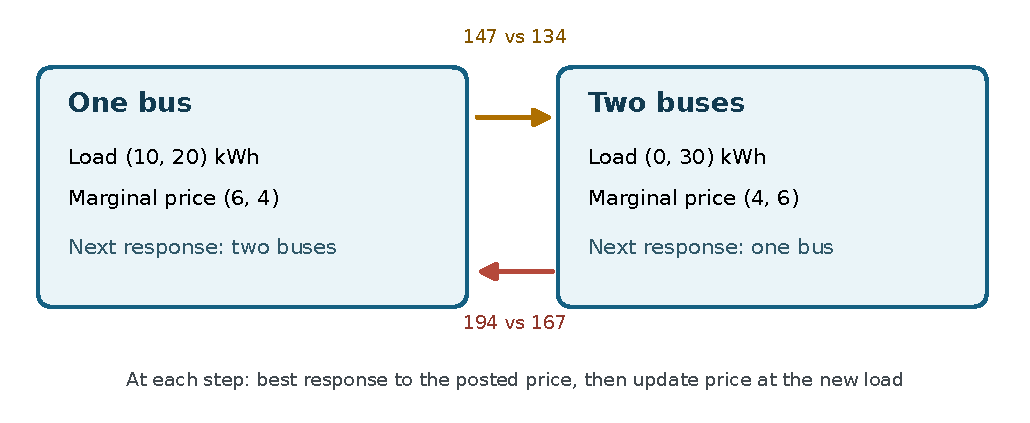
\includegraphics[width=.91\linewidth]{../figures/cyclic_price_update.pdf}
\caption{Exact undamped best-response cycle in the nominal two-service model.
Initialize at the one-bus physical optimum; each arrow holds the displayed
price fixed for the response, then updates to the marginal price of the new
load. Numbers on arrows compare the current fleet's bill with the responding
fleet's bill, in synthetic units.}
\label{fig:exact-cycle}
\end{figure}

\begin{figure}[t]
\centering
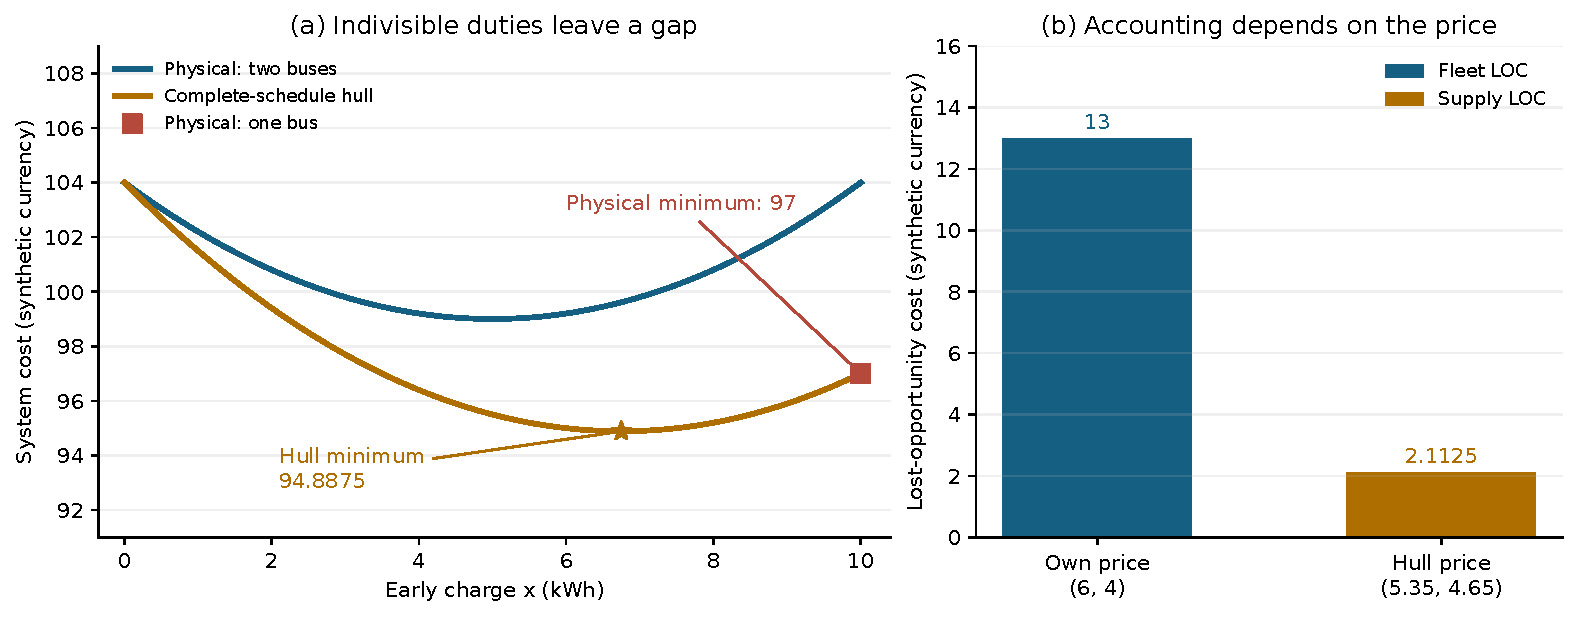
\includegraphics[width=.91\linewidth]{../figures/cyclic_gap_and_prices.pdf}
\caption{Exact physical branches, complete-fleet hull, and lost-opportunity
accounts in the synthetic two-service case.  Prices are synthetic units/kWh;
the hull mean is not an executable daily fleet.}
\label{fig:exact-gap}
\end{figure}

The binding 10 kW early limit is a fragile nominal parameter: at the same
20 kWh capacity, a positive reserve or charging loss can remove the
one-bus branch.  A nearby construction allows those constraints while
retaining a gap.  Keep two 15 kWh services, battery capacity 20, and
\eqref{eq:exact-supply}, but use reserve $r=1$ kWh, grid-to-battery
efficiency $\eta=19/20$, 12 kW individual and shared early power, and a
single 30 kW terminal connector.  The one-bus plan buys $220/19$ grid kWh
early and 20 terminally, with battery states
$20\to5\to16\to1\to20$.  Its early power has $8/19$ kWh of headroom.
The supporting two-bus plan buys $30/19$ early and 30 terminally; the two
terminal sessions take $9/19$ and $10/19$ hour and fit sequentially on the
single connector.  Every used bus again finishes full.

\begin{proposition}[A positive-gap neighborhood]\label{prop:exact-robust}
Under the modified parameters,
\begin{equation}\label{eq:exact-robust}
 D=\frac{38527}{361},\qquad
 CH=\frac{2987911}{28880},\qquad
 \Delta=\frac{94249}{28880}>0.
\end{equation}
With the 30 kW terminal connector fixed, strict feasible-headroom and
optimality inequalities preserve a positive gap in an open neighborhood
of the stated reserve, efficiency, and early power.
\end{proposition}

The interval and strict-inequality proof is in
Appendix~\ref{app:theory-proofs}.  The neighborhood is conditional on this
hardware model's zero switching time, constant efficiency, and lack of
taper.  For perspective on connector adequacy, if the original lossless
case has one terminal connector of power $K\leq30$ kW, it is infeasible for
$K<20$, has zero gap for $20\leq K\leq23.5$, and has a positive gap for
$23.5<K\leq30$.  Thus the presence of one connector alone says nothing
about price support.

\subsection{Replication and the participant scale}\label{sec:exact-replication}

Replicate A and B to $n$ simultaneous copies each.  Give the fleet $n$
early 10 kW connectors and $n$ terminal 30 kW connectors.  Battery and
service energy per bus stay fixed; supply cost scales with demand as
\begin{equation}\label{eq:exact-scaled-supply}
 F_n(E,L)=4E+\frac{E^2+L^2}{10n}.
\end{equation}
If $m$ buses each cover an A--B pair, $n-m$ A-only and $n-m$ B-only buses
complete the services.  There are $2n-m$ used buses, and physical early
energy ranges over $[10m,10n]$.  Terminal sessions have an explicit
connector-feasible assignment: paired buses take $m$ connectors, while
each A-only/B-only pair can share one of the other $n-m$ terminal
connectors sequentially.  All buses return full.

\begin{proposition}[A vanishing gap with aggregate regret]
\label{prop:exact-replication}
The complete projected hull has lower operating-cost boundary
$14n-0.7E$ and optimum $CH_n=7591n/80$.  Every physical optimum takes an
integer $m$ nearest to $27n/40$; both neighboring integers are retained at
a tie.  With $\delta=m-27n/40$,
\begin{equation}\label{eq:exact-replication-gap}
 \Delta_n=\frac{20\delta^2}{n}\leq\frac5n.
\end{equation}
Along $n=40k+1$, the whole-operator own-price regret is
\begin{equation}\label{eq:exact-replication-regret}
 r_n=\frac{351}{40}+\frac{169}{40n}\longrightarrow\frac{351}{40},
 \qquad
 \Delta_n=\frac{169}{80n}\longrightarrow0.
\end{equation}
For multiples of 40, both quantities are exactly zero.
\end{proposition}

The planning gap and the whole-operator incentive decouple:
$\Delta_n=O(1/n)$, yet $r_n$ stays bounded away from zero along
$n=40k+1$. Both are bounded independently of $n$ in this family, but only
the gap vanishes along that subsequence. Regret per bus and regret as a
fraction of physical cost also vanish. Shapley--Folkman theory explains why
sums of small nonconvex participants can become approximately convex
\citep{starr1969,hreinsson2021}; the exact rates here show why a small
planning gap alone does not control the absolute incentive of the operator
that owns the entire sum.

Now divide ownership among $n$ operators, each with one A/B service pair
and reserved early and terminal connectors. Each can choose the one-bus
plan or any two-bus plan with $x\in[0,10]$, and these deviations remain
compatible with the others' connector rights. At the physical optimum's
marginal price, each participant's regret is at most $20/n$. Their regrets
sum to the whole-fleet regret in this symmetric construction. Along
$n=40k+1$, each dissatisfied one-bus owner can gain only $13/n$, even
though their total gain tends to $351/40$. At $n=20$, the two tied planner
optima have whole-fleet regrets 7 and 14.

With separate ownership, each participant becomes negligible relative to
the growing market and its incentive vanishes. This is a small-participant
analogue of the divisible traffic flows coordinated by
\citet{alizadeh2016coupled}. With common ownership, the operator can instead
change the entire fleet at once. These two ends of the participant scale
connect the aggregation argument to the coordination model in
Section~\ref{sec:generation}; they do not identify the reserved-connector
model with Alizadeh et al.'s transportation network.

\begin{figure}[t]
\centering
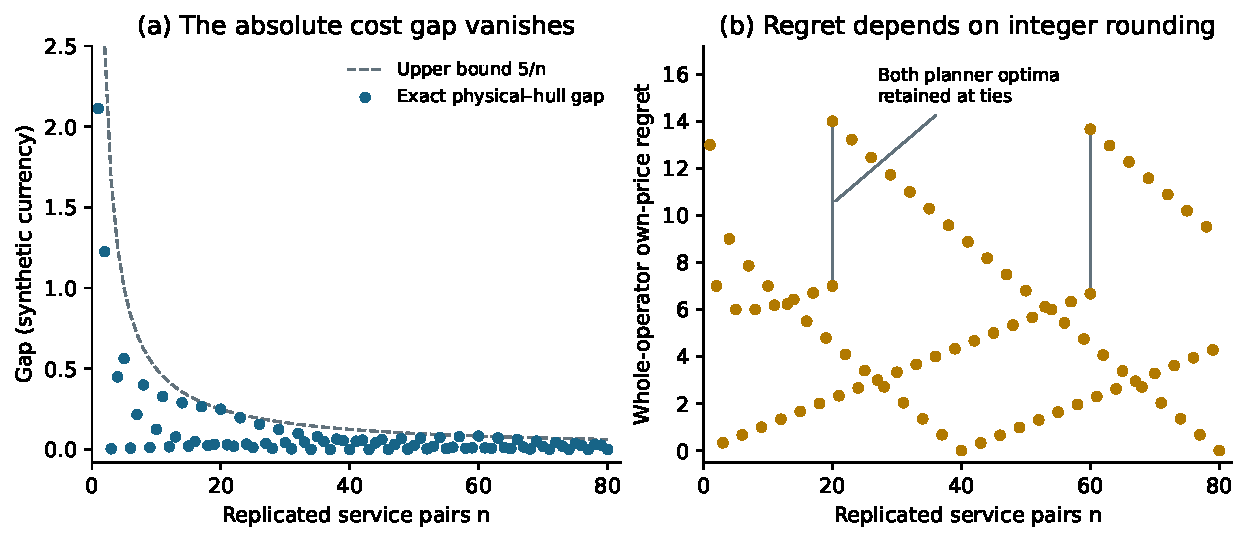
\includegraphics[width=.91\linewidth]{../figures/cyclic_replication.pdf}
\caption{Exact replication for $n=1,\ldots,80$, including both physical
optima at ties.  The planning gap follows the $5/n$ bound while
whole-operator own-price regret varies with integer rounding.  Values are
synthetic units, not observations from a bus system.}
\label{fig:exact-replication}
\end{figure}

\section{A public timetable: feasible fleets and bounded costs}\label{sec:public}

The exact two-service example isolates the mechanism; it does not measure
its prevalence or size in service.  For a timetable-scale check we use the
published Hildenbrand instance from the Sistig electric-bus scheduling data
\citep{sistig2025dataset,sistig2025electrification}: 37 mandatory services
with a complete directed deadhead matrix.  We form
two \emph{separate} one-depot cases, using depot 15 or depot 16.  These are
declared modifications of the source network, not a reconstruction of its
two-depot, multiple-output charging design.  Timetable and directed travel
times retain their source offsets, including the next-day services.  Matrix
travel times depend on origin and destination, not on departure time.

Energy and monetary inputs are explicit scenario assumptions, not observed
vehicle telemetry or source objective coefficients.  Service energy is
$1.20$ kWh/km plus 16 kWh per service hour.  Directed deadheads use
$0.96$ kWh/km plus 16 kWh per travel hour, and explicit off-depot waiting
uses 16 kWh/h; depot-parked auxiliary draw is zero.  Each used bus has
400 kWh usable inventory, zero additional reserve, unit charging
efficiency, and a 360 kW acceptance limit.  One 360 kW connector is shared
at the selected depot.  All used buses start full and return full by a
synthetic 30:00 service-block boundary.  Charging has no taper and no
switching time.  This finite block does not establish a repeating daily
operation.  A 37-bus one-service-per-bus construction confirms feasibility
of both cases, but has no optimization role.  Monetary travel cost is zero:
the objective charges the used-bus fee and grid energy, while movement
energy and time remain in the physical constraints.

We first use synthetic used-bus cost $f=100$ and flat grid price
$a=0.2$ per kWh.  Because this objective is linear in load, minimizing it
over the hull of complete plans has the same value as minimizing it over
physical plans; this flat-price experiment cannot exhibit a physical--hull
gap.  The original fixed-budget native runs returned physically replayed
two-bus schedules in both depot cases without proving objective optimality.
A separate, already archived round-0 solve
within the later nonlinear planner used the same complete depot-15 physical
case and a tangent objective that reduces exactly to the flat price.
That call returned a \emph{native numerical} optimum of approximately
408.53, with matching incumbent and lower bound under solver tolerances.
This is a retrospective interpretation of one call, not a new flat-price
experiment or a reclassification of the nonlinear campaign.  The numerical certificate does not identify the exact rational-model
optimum.  The following ideal stored-input certificates answer that
distinct exact-arithmetic question.

For both depot graphs, a one-bus path is impossible.  Chronologically
forced adjacent services leave no admissible depot visit, while mandatory
service energy alone exceeds one bus's 400 kWh inventory.
An exact cardinality-gated path-cover relaxation of each full 37-service
graph gives flat-objective lower bounds displayed outward as 404.92 at depot
15 and 414.39 at depot 16.  The bounds retain every declared connection
mode but relax some physical constraints.  Separately, an exact rational
depot-15 witness covers all 37 services with two buses, respects the shared
connector, and restores both batteries to 400 kWh by 30:00.  Hence depot 15's ideal
model has a minimum fleet of two and the \emph{flat-cost optimum} lies in
\begin{equation}\label{eq:public-flat}
 D^{\rm flat}_{15}\in[404.92,408.54]
 \quad\text{(outward-rounded exact rational bounds).}
\end{equation}
The bounds do not identify the optimum.  Depot 16 has the exact
at-least-two obstruction and lower bound, but its returned two-bus upper
witness remains numerical, yielding a mixed-evidence interval
$[414.39,433.75]$ after outward rounding.  In
particular, a native solver's rounded matrix and its feasibility tolerances
are distinct from the ideal stored-input rational model.

For a nonlinear illustration on \emph{the same finite depot-15 ideal
model}, let $e_t$ be hourly grid energy for 30 market intervals and set
\begin{equation}\label{eq:public-quadratic}
 F(e)=\sum_{t=1}^{30}\left(0.2e_t+\frac{e_t^2}{1800}\right).
\end{equation}
The coefficients and bus cost remain synthetic.  The exact two-bus witness
gives a physical upper bound displayed as 512.77.  To bound the complete
hull from below, let $L_{\rm flow}$ denote the exact depot-15 two-path
flat-cost relaxation value.  Because monetary travel cost is zero, it
implies at least $E_{\min}=(L_{\rm flow}-2f)/a\approx1024.62$ kWh for any
two-bus plan.  One bus is impossible, and a uniform-price comparison using
the service-energy floor excludes three-or-more-bus plans from improving the
dual lower certificate.  The 30-period Fenchel inequality then gives the
exact rational lower bound displayed as 424.36.  Therefore
\begin{equation}\label{eq:public-nonlinear}
 424.36\leq CH_{15}\leq D_{15}\leq512.77,
 \qquad 0\leq D_{15}-CH_{15}\leq88.41.
\end{equation}
All displayed endpoints are rounded outward from the exact bounds.  They
do not establish $CH_{15}$ or $D_{15}$ individually, nor a strictly positive
gap.  The public case thus demonstrates physically feasible complete-fleet
witnesses and useful bounds under declared assumptions, while leaving
public price support open.


\begin{figure}[t]
\centering
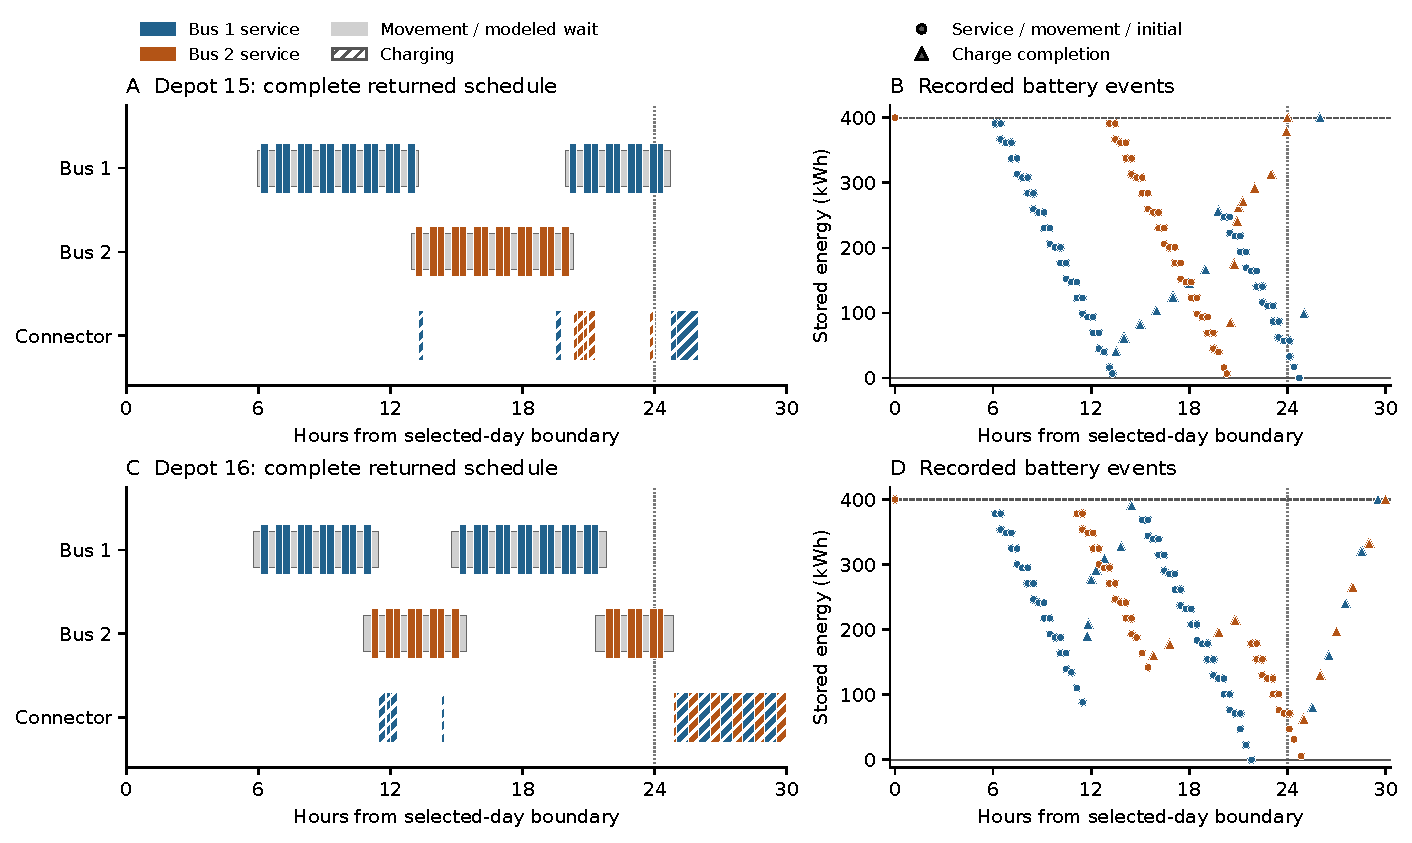
\includegraphics[width=\linewidth]{../figures/public_pilot_witnesses.pdf}
\caption{Two-bus schedules returned by the original flat-price pilot for
the two depot variants of the same Hildenbrand timetable.  Battery and
charging traces describe numerical feasible witnesses under the declared
scenario assumptions.  They are not measured operation, two independent
networks, or proofs of cost optimality.  The separately constructed exact
depot-15 witness supplies the ideal-model bounds in the text.}
\label{fig:public-witnesses}
\end{figure}

\section{Computational evidence}\label{sec:computational}

The computations ask whether complete-fleet convexification can be bounded at a changed supply market, and which parts of repeated optimization remain costly.  They do not estimate a population-level speedup.  We use two deliberately small synthetic cases and two depot variants of a single 37-service Hildenbrand timetable.  Depot 15 and depot 16 use different depots in that base network; they are not independent public replications.  The reported results come from one run of each campaign.  The campaigns reuse cases, code paths, and in some instances source-plan evidence, so their cells cannot be pooled as independent trials.

For a case $I$, let $\mathcal F(I)$ be its set of \emph{complete} physically feasible fleet schedules.  A column $x\in\mathcal F(I)$ includes the service assignment, vehicle paths, charging decisions, and full-horizon load $e(x)$, with operating cost $c(x)$.  For the separable quadratic supply model
\begin{equation}\label{eq:computational-supply}
 G_s(e)=\sum_{t=1}^{T}\left(a_{s,t}e_t+\tfrac12 b_t e_t^2\right),\qquad s\in\{0,1\},
\end{equation}
the pure-fleet and complete-fleet-hull objectives are
\begin{equation}\label{eq:computational-D-CH}
\begin{aligned}
 D_s&=\min_{x\in\mathcal F(I)}\{c(x)+G_s(e(x))\},\\
 CH_s&=\min_{(e,c)\in\operatorname{conv}\{(e(x),c(x)):x\in\mathcal F(I)\}}\{c+G_s(e)\}.
\end{aligned}
\end{equation}
State 0 is the source market and state 1 is the changed target market on the \emph{same} physical case.  In the public cases $T=30$, $b_t=1/900$, and $a_{0,t}=0.20$ throughout; the target has $a_{1,t}=0.18$ in the first 15 periods and $0.22$ in the last 15.  The synthetic cases have four periods and similarly paired source and target coefficients.  This controlled price change makes same-case reuse meaningful without treating a source-market solution as a target-market optimum.

We report an interval $[L,U]$ for $CH_1$ only when the run produced the required evidence.  Its upper endpoint is the objective of a feasible \emph{convex mixture} of complete fleet columns.  That mixture is a valid hull point, but generally cannot be dispatched as one fleet schedule.  A global lower endpoint is assembled from physical fleet-pricing evidence in the target market, including checked inherited physical-pricing bounds where explicitly indicated.  Native mixed-integer solver bounds and replayed numerical solutions retain the solver's tolerance qualifications; they are computational enclosures, not exact proofs for the ideal model.  A zero or small gap in the finite \emph{restricted} column pool does not close the global interval: ungenerated complete fleets still matter.  Nor does an interval for $CH_1$ alone establish the pure-fleet value $D_1$, a nonconvexity gap $D_1-CH_1$, or support by any proposed tariff.

\begin{table}[t]
\centering\small
\caption{Development campaigns and their declared scope.  Outcomes count cells for the two iterative-hull campaigns and fixed-price calls for the pricing-start campaign.  The same four physical cases recur across campaigns.}\label{tab:computational-scope}
\begin{tabular}{>{\raggedright\arraybackslash}p{0.20\linewidth}>{\raggedright\arraybackslash}p{0.35\linewidth}>{\raggedright\arraybackslash}p{0.36\linewidth}}
\toprule
Campaign & Design & Observed outcomes \\
\midrule
Feasible-pool pilot & Three hull methods $\times$ four cases $\times$ two markets; reserve and source-column reuse & 24 cells: 7 certified and 17 budget-exhausted.  Both public target depot variants remained open. \\
Solver-baseline comparison & Four ordered hull methods $\times$ four cases $\times$ two markets; numerical restricted master and physical-bound cache & 32 cells: 11 certified, 18 budget-exhausted, 3 failed.  No public target cell certified. \\
Pricing-start pilot & Cold versus submitted movement start at two fixed price queries on four cases & 16 calls returned.  Four synthetic pairs agreed within tolerance; all eight public calls reached the native 160-s cap. \\
\bottomrule
\end{tabular}
\end{table}

\subsection{Complete-fleet hull updates}

The first pilot compared a legacy cold run, a cold run that reserves time for a subsequent restricted master, and that reserve policy with feasible source-column reuse.  The reserve made a second master possible in all four public reserve-cold cells, while the corresponding legacy cells ended after one master.  In the changed market, the reuse method admitted two feasible state-0 columns to its first master, obtained one fresh target-market priced column, and processed it in a second master.  The source columns help form target-market feasible mixtures, but they do not replace target-market pricing for a global lower bound.

On the synthetic cyclic case, all six market-by-method cells certified.  On the multivisit case, the source market exhausted its budget in all three methods.  In the target market, reuse closed the global enclosure while the two cold methods exhausted their budgets: its displayed interval is $[84.72,84.73]$ after outward rounding, versus $[81.17,86.05]$ for reserve cold.  This is a diagnostic of the method under the declared small-case budget, not a claim about larger networks.

For the public target cases, reserve cold lowered the feasible upper relative to legacy cold, from $547.47$ to $526.31$ at depot 15 and from $549.70$ to $531.90$ at depot 16.  Reuse lowered those upper endpoints further to $469.89$ and $490.67$.  Yet its fresh global lower endpoints were $315.76$ and $329.22$, below reserve cold's $339.35$ and $377.65$.  Thus the upper improvements of $56.43$ and $41.24$ do not imply tighter \emph{global} enclosures; in depot 16 the interval width actually grows.  The public reuse cells stopped at projected rational-polishing bit growth, whereas reserve-cold cells stopped at the explicit pricing-reserve guard.

The ordered solver-baseline comparison then retained feasible columns and introduced two further mechanisms.  A numerical quadratic-program (QP) \emph{restricted-master proposal} selects mixture weights over the currently known complete-fleet columns; a checked rational replay admits its objective and residual.  The fourth method also re-evaluates an inherited \emph{physical-pricing lower bound} under the changed market's Fenchel conjugate.  This cache concerns already-checked physical pricing evidence, not a cache of an unverified schedule or a substitute for all fresh target-market pricing.  Table~\ref{tab:public-hull} gives all public target outcomes in this comparison, including the paid source-state work and source-admission cost for retained methods.

\begin{table}[t]
\centering\small
\caption{Public target-market hull evidence in the ordered solver-baseline comparison.  $L$ is rounded down and $U$ up to two decimals; unrounded stored values determine certification.  ``Exhausted'' means budget exhausted.  Paid time includes both market states and, where applicable, parent source admission.  A failed target has no final interval even though its time was paid.}\label{tab:public-hull}
\begin{tabular}{llrrrr}
\toprule
Depot & Method & $L$ & $U$ & Paid (s) & Outcome \\
\midrule
15 & Reserve cold & --- & --- & 347.20 & failed \\
15 & Reserve + pool & 315.76 & 469.89 & 354.61 & exhausted \\
15 & QP + pool & --- & --- & 349.88 & failed \\
15 & QP + pool + cache & 405.83 & 471.52 & 352.27 & exhausted \\
\addlinespace
16 & Reserve cold & 377.65 & 531.90 & 351.08 & exhausted \\
16 & Reserve + pool & 350.87 & 490.67 & 353.48 & exhausted \\
16 & QP + pool & --- & --- & 349.53 & failed \\
16 & QP + pool + cache & 420.45 & 491.46 & 352.22 & exhausted \\
\bottomrule
\end{tabular}
\end{table}

\begin{figure}[t]
\centering
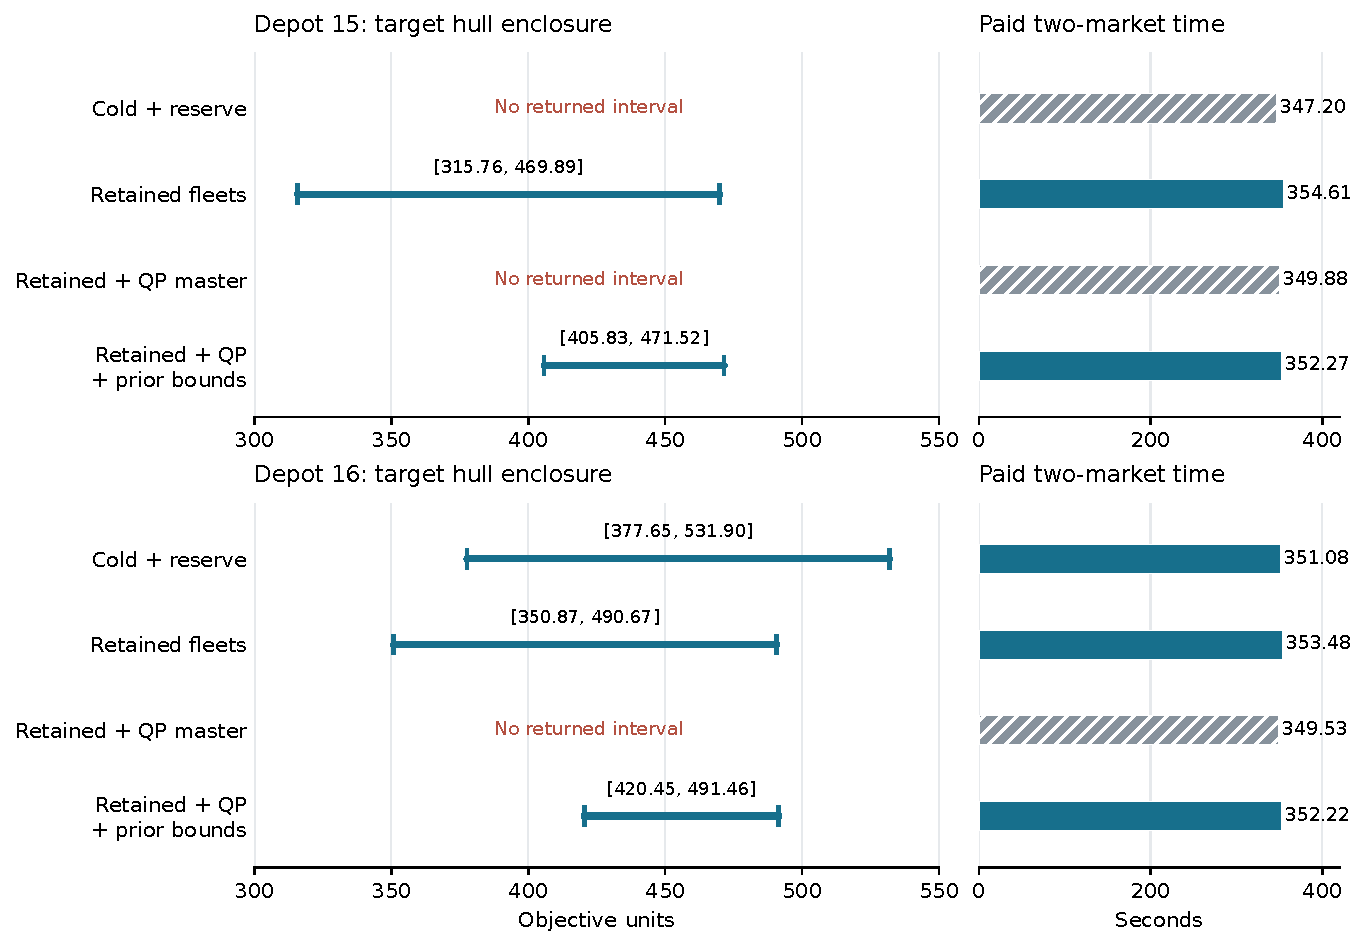
\includegraphics[width=\linewidth]{figures/public_hull_comparison.pdf}
\caption{All eight public target cells in the ordered solver-baseline comparison: global hull intervals and paid two-market cost.  Lower endpoints use physical-pricing evidence and upper endpoints feasible mixtures.  Every completed interval remains open.  Hatching marks a failed target with no final bound interval; its spent time remains in the paid-cost panel.  The depot variants share one timetable.}\label{fig:public-hull}
\end{figure}

The completed public QP-and-cache cells ended with restricted-pool residuals below the configured $10^{-6}$ pool tolerance, without exhausting the rational-polishing bit budget.  Their \emph{global} intervals were still open by $65.68$ and $71.00$ objective units, and both stopped on native remaining-time budget.  In each, one fresh physical target pricing result was recorded.  The inherited, target-revalued physical lower exceeded the best fresh lower within the same run by $98.82$ at depot 15 and $69.83$ at depot 16; the selected global lowers were $405.83$ and $420.45$.  This within-run decomposition identifies a useful source of bound strength.  It cannot isolate a causal cache effect across methods: the QP-without-cache target cells failed, and the cached method also incurs source-state computation and admission work.

An implementation error when a pricing call returned no incumbent caused three target failures: depot 15 reserve cold and both depot variants with the numerical restricted master and pool but no bound cache.  No new completed pricing result or global bound was produced for the failing call.  Their spent time remains in Table~\ref{tab:public-hull}, and their missing intervals cannot be imputed from another method.  On the two synthetic cases, all methods certified cyclic in both markets, while the three retained-pool methods certified multivisit in the changed market and reserve cold did not.

The iterative timings explain why a faster restricted master alone would have limited impact on these public cells.  Recorded successful public physical-pricing calls were about 160~s, while QP proposal took $0.77$--$1.07$~s and rational replay $0.51$--$0.53$~s in the completed cached targets.  The feasible-pool pilot's public changed-market pricing consumed roughly 160--172~s per cell; its master native solves were below $0.01$~s, though rational polishing in reuse took about six seconds.  Component scopes differ and may overlap, so these quantities are not an additive time budget.  In the first pilot, paid source-plus-target times were about 369~s for legacy cold, 350~s for reserve cold, and 351--352~s for reuse on the public variants.  Those methods ended at different bounds and stopping points.  Neither campaign specified an equal-quality time target, and none of these differences is an equal-quality speedup estimate.

\subsection{Fixed-price movement starts}

The separate pricing-start pilot probes the physical pricing oracle at fixed prices rather than running the iterative hull.  Its \emph{linear} query uses the target market's coefficients $p_t=a_{1,t}$.  Its \emph{marginal} query uses $p_t=a_{1,t}+b_te_t(\bar x)$, where $\bar x$ is the cheapest linear-bill schedule among the common feasible source columns.  This anchor is a selected feasible column, not a certified target planner optimum.  The two price vectors are distinct in all four cases.  A common feasible source schedule supplied a baseline upper to both arms; the start arm additionally submitted its checked discrete movement selections to the native solver, leaving continuous charging as a solver decision.  Submission was observed, but native acceptance or use of the hint was not.

The four synthetic pairs returned the same certified numerical intervals under cold and submitted-start calls, within the comparison tolerance.  Table~\ref{tab:pricing-start} reports the four public pairs.  Every public native call ran to the 160-s cap and returned a physically replayed incumbent.  On depot 15's marginal query the start improved that incumbent by $1.10$ but worsened the admitted lower by $3.59$.  On depot 16's marginal query the incumbent tied while the admitted lower improved by $11.78$.  The depot 15 linear lower worsened by $5.68$, and the depot 16 linear pair tied.  These crossed upper/lower movements give no consistent bound-quality improvement.

\begin{table}[t]
\centering\small
\caption{Public fixed-price pricing at the same native 160-s cap.  Each pair has a common feasible source upper.  The displayed lower is the admitted native lower (rounded down); the displayed upper is the physically replayed native incumbent (rounded up).  ``Paid'' is the complete child time for cold/start, not just native optimization.}\label{tab:pricing-start}
\begin{tabular}{llrrrrr}
\toprule
Depot & Price & Cold $L$ & Cold $U$ & Start $L$ & Start $U$ & Paid cold/start (s) \\
\midrule
15 & linear & 345.86 & 413.67 & 340.18 & 413.67 & 163.01 / 163.31 \\
15 & marginal & 383.00 & 419.06 & 379.41 & 417.95 & 163.15 / 163.25 \\
16 & linear & 377.65 & 430.86 & 377.65 & 430.86 & 163.11 / 163.20 \\
16 & marginal & 416.72 & 438.17 & 428.51 & 438.17 & 163.11 / 163.17 \\
\bottomrule
\end{tabular}
\end{table}

\begin{figure}[t]
\centering
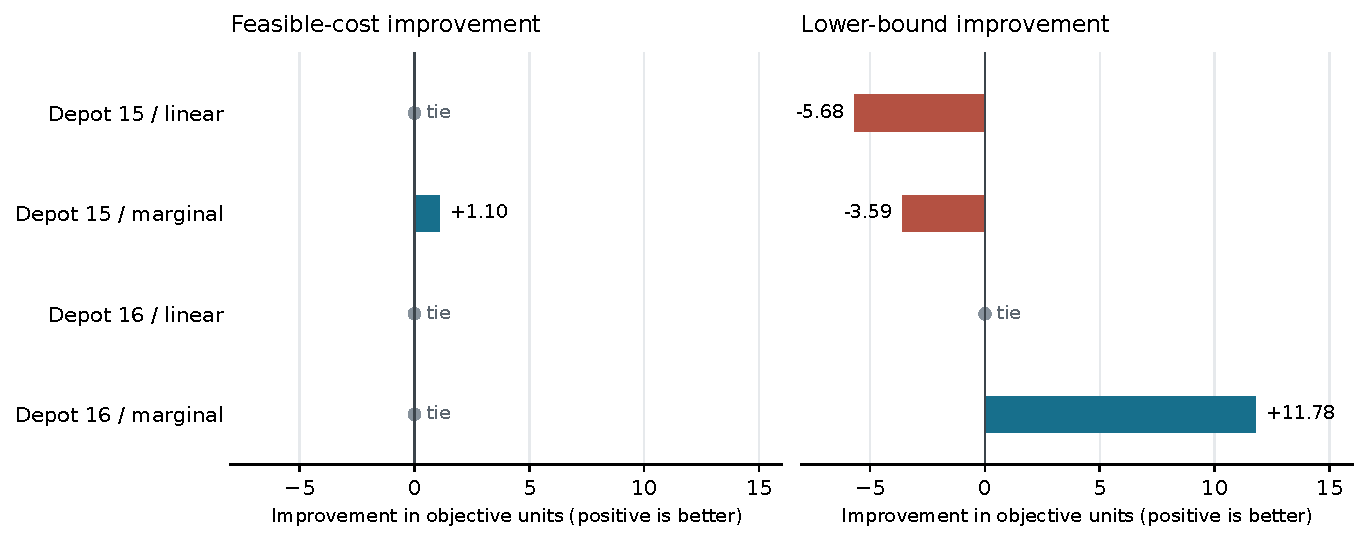
\includegraphics[width=\linewidth]{figures/pricing_start_effects.pdf}
\caption{Within-pair public effects of a submitted movement start on replayed incumbent and admitted lower bound at fixed native caps.  A smaller incumbent and a larger lower bound are favorable; the effects differ by query and depot.}\label{fig:pricing-start}
\end{figure}

The historical construction of the four shared source pools cost $358.21$~s once.  The preparation command, including source admission, cost a further $1.96$~s.  The 16 complete child receipts sum to $1{,}317.51$~s; adding the once-paid source work and freeze command gives $1{,}677.67$~s for this source-inclusive accounting.  Nested native, setup, and child timings must not be added again.  The source schedule was only modestly worse than the best newly returned public incumbent at this cap, with excess ranging from $0.32\%$ to $2.74\%$ of that returned incumbent's fixed-price objective.  This denominator is a feasible result, not the unknown fixed-price optimum.  No time to first incumbent was recorded, so the observed equal-cap quality cannot be converted into a start-induced time-to-solution claim.

\subsection{What the experiments establish}

\begin{table}[t]
\centering\small
\caption{Evidence map for the computational claims.  ``Established'' refers to the declared development cells and native-tolerance-qualified intervals, not to independent statistical replication.}\label{tab:computational-evidence-map}
\begin{tabular}{>{\raggedright\arraybackslash}p{0.30\linewidth}>{\raggedright\arraybackslash}p{0.60\linewidth}}
\toprule
Established in these cells & Still untested or unresolved \\
\midrule
Complete-fleet feasible columns can be reused across the two markets, and the multivisit target enclosure closed under reuse. & Whether reuse improves target-market global gaps or paid time across independent public timetables at equal quality. \\
Checked inherited physical-pricing evidence strengthened the selected lower in two completed public cached runs. & A causal cache effect against a completed, equally budgeted QP-without-cache target and a public global certification. \\
Movement starts were submitted and public fixed-price calls returned mixed incumbent/lower effects at equal native caps. & Native hint acceptance, time to first incumbent, and any robust start-induced speedup or learned-proposal benefit. \\
\bottomrule
\end{tabular}
\end{table}

The open public global intervals therefore remain the central computational limit for price support: a nearly solved restricted pool does not determine the full fleet hull or certify a target-market tariff.  Nearest-neighbor retrieval and learned proposals remain untested here; evaluation across independent timetable groups is future work.


\section{Implications and limits}
The analytical and computational parts answer complementary questions. The construction proves that continuous charging and full replenishment do not remove the possibility of a marginal-price support failure. The experiments measure how difficult it is to obtain informative full-fleet bounds on declared instances. An unresolved public interval neither confirms the analytical mechanism on that timetable nor refutes it. Likewise, a strong restricted-master solution says little about the cost of discovering an ungenerated physical fleet unless global pricing has supplied a corresponding bound.

This distinction informs the route toward faster online decisions. Retained complete fleets already provide feasible candidates after a price-only change when the physical case remains unchanged. A nearest-neighbor proposal or a learned route predictor should first be compared against that baseline and against choosing the cheapest current bill from the same stored pool. Route fragments require assembly and physical repair before becoming a complete feasible fleet. Evaluation should report direct proposal quality, repair effort and optional global verification separately; a good dispatch need not come with a global optimality certificate. Training-data generation and source optimization are costs, even when amortized over later queries.

The present studies do not evaluate those retrieval or learned methods. They also do not establish transfer across timetables, demand regimes or charger designs. Future comparisons must keep all depot, tariff and timing variants of a base timetable within one data group and reserve independent timetables before training. Time-limited incumbents should retain their bound gaps instead of becoming exact labels. Repeated seeds, independent cases and time-to-common-quality targets would be needed before interpreting runtime differences as systematic acceleration.

The physical model abstracts from stochastic delays, battery degradation, temperature-dependent consumption, nonlinear charging taper and operational switching times. Public service and travel inputs are combined with declared energy and economic assumptions; the results are not estimates of savings for the source operator. Resource rights also delimit the economic interpretation. A whole-fleet price-taking deviation, an individually reserved-pair deviation and a strategic operator anticipating its own price impact are different optimization problems. Conclusions must follow the chosen participant and settlement model.

\section{Conclusion}
A smooth convex electricity supply cost need not support an indivisible electric-bus fleet at its own marginal prices. A fully replenished construction exhibits this failure and retains it under a specified robust variant. Replication can make the planning gap small without making the incentive of one whole-fleet operator small along every subsequence, while incentives for reserved pairs vanish. Development computations show that feasible-fleet reuse and inherited pricing bounds can help particular solves, but fresh global pricing remains costly and public gaps remain open. The current evidence supports further controlled computational work; it does not yet establish a learned method or general online acceleration.

\section*{Data and reproducibility}
The \href{https://github.com/ndandnd/egg}{EGG research repository} contains the analytical constructions, declared public-data transformation, experiment protocols, complete outcome tables including unsuccessful attempts, and figure-generation sources. A companion source map links the manuscript's claims to reviewed evidence and distinguishes exact ideal-model calculations from tolerance-qualified native results. All cases reported here are development cases. No private operational data or reserved evaluation outcomes are used. The figures in this manuscript are drawn from already reviewed results; its assembly required no new optimization. The supplementary research record retains execution and qualification details without treating those checks as empirical performance results.

\appendix
\section{Proofs for the complete-fleet statements}\label{app:theory-proofs}

\begin{proof}[Proof of Proposition~\ref{prop:theory-support}]
For physical $x$, $p\in\partial F(e(x))$, and any hull point $(e,c)$,
linear minimization over the convex hull gives
$c+p^\top e\geq V(p)$.  The subgradient inequality gives
$F(e)\geq F(e(x))+p^\top(e-e(x))$.  Adding and minimizing over the hull
yields $CH\geq c(x)+F(e(x))-r(x;p)$, proving the first inequality;
$c(x)+F(e(x))\geq D\geq CH$ proves the second.  If $r(x;p)=0$, all
inequalities collapse to $CH=D=c(x)+F(e(x))$.  Conversely, compactness
supplies a physical minimizer when $D=CH$.  Under the relative-interior
condition, Fenchel--Rockafellar duality gives an attained maximum
$CH=V(p^*)-F^*(p^*)$.  Under the alternative minorant condition, apply
the same duality theorem to that finite minorant.  It agrees with $F$
on all hull loads, while its conjugate bounds $F^*$ from above; weak
duality for $F$ then makes the same $p^*$ optimal for $F$.  For any
physical minimizer $x^*$, the two
nonnegative Fenchel terms satisfy
\[
r(x^*;p^*)+
F(e(x^*))-(p^*)^\top e(x^*)+F^*(p^*)
=D-CH=0.
\]
Each term is therefore zero.  Fenchel equality gives
$p^*\in\partial F(e(x^*))$ and the first equality gives
$r(x^*;p^*)=0$.  This holds for every physical minimizer and every
attained hull-dual maximizer.
\end{proof}

\begin{proof}[Proof of Corollary~\ref{cor:best-price}]
Let $(e^*,c^*)$ be a hull minimizer with $e^*=e(x)$, and let $p^*$ be an
attained hull-dual maximizer. The nonnegative terms
$c^*+(p^*)^\top e^*-V(p^*)$ and
$F(e^*)-(p^*)^\top e^*+F^*(p^*)$ sum to zero by strong duality.
Hence $p^*\in\partial F(e^*)$ and
$r(x;p^*)=c(x)-c^*=c(x)+F(e(x))-CH=H(x)$.
Proposition~\ref{prop:theory-support} supplies the matching lower bound
for every price in $\partial F(e(x))$.
\end{proof}

For the accounting identity, $F^*(p)\geq p^\top e(x)-F(e(x))$ by
definition, so supplier LOC is nonnegative.  Substitution in
\eqref{eq:theory-loc} gives the claimed sum.  The same
qualification above yields an attained hull-dual price
$p^*$ and $V(p^*)-F^*(p^*)=CH$.  At a physical planner optimizer the
LOC sum is $D-CH$.  At any price in the plan's subdifferential, Fenchel
equality makes supplier LOC zero.

\begin{proof}[Proof of \eqref{eq:theory-upper}]
Let $(e^*,c^*)$ be a hull minimizer, $p^*=a+Qe^*$,
$d=\|e(x)-e^*\|_Q$, and $H=H(x)$.  First-order hull optimality makes
$(e^*,c^*)$ a minimizer of $c+(p^*)^\top e$, so
\[
 \mathrm{LOC}_{\rm fleet}(x;p^*)=H-\tfrac12d^2\geq0.
\]
In particular $d\leq\sqrt{2H}$.  For each physical alternative $y$,
the change in its linear advantage when the price moves from $p^*$ to
$p_x=p^*+Q(e(x)-e^*)$ is
$(e(x)-e^*)^\top Q(e(x)-e(y))$, at most $dR_Q$ by
the seminorm Cauchy--Schwarz inequality.  Maximizing over $y$ gives
$r(x)\leq H-d^2/2+dR_Q\leq H+R_Q\sqrt{2H}$.
The lower inequality is Proposition~\ref{prop:theory-support}.
\end{proof}

\begin{proof}[Proof of Proposition~\ref{prop:exact-nominal}]
Let $\lambda$ be the one-bus mixture weight and $x$ the mean early load.
Complete-plan mixtures have $0\leq\lambda\leq1$,
$10\lambda\leq x\leq10$, and intrinsic cost $14-7\lambda$.
These conditions are sufficient: for $\lambda<1$ the two-bus component
buys $(x-10\lambda)/(1-\lambda)\in[0,10]$ early; at $\lambda=1$,
$x=10$.  For fixed $x$, cheapest intrinsic cost uses
$\lambda=x/10$.  Substituting $z=30-x$ into \eqref{eq:exact-supply}
gives hull objective
\[
 14-\frac{7x}{10}+F(x,30-x)
 =104-2.7x+0.2x^2
 =\frac{7591}{80}+\frac{(x-27/4)^2}{5}.
\]
Its minimizer is $x=27/4$, $\lambda=27/40$.  Direct minimization of
the one- and two-bus physical branches gives respectively 97 and 99.
At $(10,20)$ the gradient of $F$ is $(6,4)$; its private objective is
$7+6(10)+4(20)=147$, while the two-bus $x=0$ plan has
$14+4(30)=134$.  At hull load $(27/4,93/4)$ the gradient is
$(107/20,93/20)=(5.35,4.65)$.  Both supporting plans have private
objective 153.5, and $F^*(p)=58.6125$ on $\R_+^2$.
The hull dual value is therefore 94.8875.  The physical one-bus plan is
a price minimizer, so fleet LOC is zero; supplier LOC is $97-94.8875$.
\end{proof}

\begin{proof}[Proof of Proposition~\ref{prop:exact-robust}]
For reserve $0\leq r\leq5$, efficiency $\eta$, one-hour early limit
$P$, and one-hour single terminal connector $K$, write
\[
 T=30/\eta,\quad \ell=\max\{0,T-K\},\quad
 u=\min\{P,15/\eta\},\quad
 h=\max\{\ell,(10+r)/\eta\}.
\]
The two-bus physical early-energy interval is $[\ell,u]$, and the
one-bus interval is $[h,u]$ when nonempty.  The lower limit $\ell$
enforces terminal connector capacity, while $(10+r)/\eta$ ensures the
one bus can begin B above reserve.  For every point in these intervals,
charge only A's bus early; terminal demands total $T-x\leq K$ and can be
served serially in the one-hour terminal window.  Individual inventories
and acceptance limits hold, and all used buses finish at capacity.

Write $G_T(x)=F(x,T-x)$, $k=1/5$, and
$m=T/2-5a/2$ for early linear coefficient $a=4$.  Then
$G_T(x)=G_T(m)+k(x-m)^2$.  Suppose
$\ell<m<h<u$, $f>0$, and
$f<2k(h-\ell)(h-m)$.  The cheapest hull operating-cost boundary over
$[\ell,h]$ is $2f-f(x-\ell)/(h-\ell)$, obtained by mixing the
two-bus endpoint $\ell$ and one-bus endpoint $h$; over $[h,u]$ it is
$f$.  Put $d=h-\ell$.  The strict inequality places the hull minimum
$x^*=m+f/(2kd)$ inside $(m,h)$.  Physical branch minimization gives
\[
 D=G_T(m)+\min\{f+k(h-m)^2,2f\},\quad
 CH=G_T(m)+2f-\frac{f(m-\ell)}d-\frac{f^2}{4kd^2}.
\]
Consequently
\[
 \Delta=\min\left\{k(h-x^*)^2,
       \frac{f(m-\ell)}d+\frac{f^2}{4kd^2}\right\}>0.
\]
At $(r,\eta,P,K,f,a)=(1,19/20,12,30,7,4)$,
$(\ell,m,h,u,d)=(30/19,110/19,220/19,12,10)$.
The inequalities are strict: $u-h=8/19$ and
$2kd(h-m)=440/19>7$.  Rational substitution yields
\eqref{eq:exact-robust}.  All strict inequalities persist under small
changes in $(r,\eta,P)$ with $K=30$ fixed.
\end{proof}

\begin{proof}[Proof of Proposition~\ref{prop:exact-replication}]
For $m$ paired buses, total early energy $E$ ranges over
$[10m,10n]$, with intrinsic cost $14n-7m$ and terminal energy
$30n-E$.  Convexifying complete plans gives a triangular projected set;
its cheapest operating cost at each $E$ is $14n-0.7E$.  Substitution in
\eqref{eq:exact-scaled-supply} gives a quadratic minimized at
$E=27n/4$ with value $7591n/80$.

For fixed integer $m\geq n/2$, physical supply cost is minimized at
$E=10m$, and the total objective is
$104n-27m+20m^2/n=7591n/80+20(m-27n/40)^2/n$.
For $m\leq n/2$, the best early load is $E=5n$ when feasible and the
branch objective is $99n-7m$, decreasing toward $n/2$.  For odd $n$, moving from $m=\lfloor n/2\rfloor$ to
$m=\lceil n/2\rceil$ changes the minimized objective by $-7+5/n<0$.
For even $n$, the two formulas agree at $m=n/2$, and an integer nearest
to $27n/40$ lies in the upper regime.  Thus the nearest integer to
$27n/40$ is optimal,
with both integers at a half-integer tie and $|\delta|\leq1/2$.

At a physical optimum, the price is
$p=(4+2m/n,6-2m/n)$.  The one-bus private objective minus the best
two-bus private objective is $40\delta/n$; the latter buys zero early
energy when $m/n\geq1/2$.  Hence whole-operator regret is
\[
 r_n=\begin{cases}
 m\,40\delta/n,&\delta\geq0,\\
 (n-m)(-40\delta/n),&\delta<0.
 \end{cases}
\]
For $n=40k+1$, $m=27k+1$ and $\delta=13/40$, giving
\eqref{eq:exact-replication-regret}.  The same difference is a
reserved pair's individual regret when its current choice is worse;
$|40\delta/n|\leq20/n$.  Summing the disadvantaged pairs reproduces
the whole-operator expression because each pair has its own reserved
connector rights.
\end{proof}

\subsection{Averaged responses in the quadratic example}\label{app:averaged-responses}

Consider the exact recurrence in Section~\ref{sec:generation}, with
$\alpha_k=0.5/\sqrt{k}$ and projection onto $\R_+^2$. Put
$e_k=e(x_k)$, $c_k=c(x_k)$, $s_k=(5[p_{1,k}-4]_+,5p_{2,k})$,
$d_k=e_k-s_k$, and $A_K=\sum_{k=1}^K\alpha_k$.
The fleet loads satisfy $0\le e_{1,k}\le10$ and $20\le e_{2,k}\le30$.
For $k\ge7$, $5\alpha_k<1$. If $p_{1,k}\ge4$, its unprojected successor
is a convex combination of $p_{1,k}$ and $4+e_{1,k}/5\in[4,6]$.
If $p_{1,k}<4$, that successor is $p_{1,k}+\alpha_ke_{1,k}\in[0,6)$.
The second coordinate is a convex combination of $p_{2,k}$ and
$e_{2,k}/5\in[4,6]$. Thus projection is inactive from $k=7$ onward,
and prices, supply responses and $d_k$ remain bounded.

Summing $\alpha_kd_k=p_{k+1}-p_k$ from $k=7$ shows that
$\bar e_K-\bar s_K\to0$, where bars denote step-weighted averages.
The finite prefix has vanishing weight. Also,
\[
 \sum_{k=7}^K\alpha_kp_k^\top d_k
 =\frac12\left(\|p_{K+1}\|^2-\|p_7\|^2
                  -\sum_{k=7}^K\alpha_k^2\|d_k\|^2\right).
\]
Dividing by $A_K$ gives zero in the limit, since
$A_K\asymp\sqrt K$ and $\sum_{k=1}^K\alpha_k^2=O(\log K)$.
The projection inequality underlying \eqref{eq:dispatch-rate} gives the
stronger weighted statement
\[
 0\le\frac1{A_K}\sum_{k=1}^K\alpha_k[CH-Q(p_k)]
 \le\frac{\|p_1-p^*\|^2+M^2\sum_{k=1}^K\alpha_k^2}{2A_K}
 \longrightarrow0,
\]
with the attained price $p^*=(107/20,93/20)$ and a bound $M$ on
$\|d_k\|$. Exact oracle solutions satisfy
$c_k+F(s_k)=Q(p_k)-p_k^\top d_k$, so their step-weighted mean tends
to $CH$. Jensen's inequality, the vanishing load mismatch, and uniform
continuity of the quadratic on bounded loads now imply
\[
 CH\le\bar c_K+F(\bar e_K)
 \le\frac1{A_K}\sum_{k=1}^K\alpha_k[c_k+F(s_k)]+o(1)
 \longrightarrow CH.
\]
The averaged fleet point belongs to the compact complete-fleet hull.
Its unique optimizer therefore gives
$(\bar e_K,\bar c_K)\to((27/4,93/4),371/40)$.
Since $c_k$ equals 7 for one bus and 14 for two,
$\bar c_K=14-7\bar w_K$, where $\bar w_K$ is the step-weighted one-bus
frequency. Hence $\bar w_K\to27/40$. An eventually constant bus count
would instead give zero or one, so both counts occur infinitely often.

This proof concerns the stated quadratic recurrence and exact responses.
It does not apply a square-summable-step theorem to $1/\sqrt{k}$ steps,
or assert recovery of a physical fleet from its convexified average.

\FloatBarrier
\bibliographystyle{plainnat}
\bibliography{references}
\end{document}
